\documentclass[journal=jpcbfk,manuscript=article,layout=singlecolumn,articletitle=true]{achemso}
\setkeys{acs}{articletitle = true}
%%%%%%%%%%%%%%%%%%%%%%%%%%%%%%%%%%%%%%%%%%%%%%%%%%%%%%%%%%%%%%%%%%%%%
%% Place any additional packages needed here.  Only include packages
%% which are essential, to avoid problems later.
%%%%%%%%%%%%%%%%%%%%%%%%%%%%%%%%%%%%%%%%%%%%%%%%%%%%%%%%%%%%%%%%%%%%%
\usepackage{graphicx,bm,lineno,mathpazo}  
\usepackage{amssymb,amsfonts,amsmath,mathtools}
\usepackage{algorithm,algpseudocode,booktabs,dcolumn}
\captionsetup{labelfont=bf}
\usepackage[input-decimal-markers={.},separate-uncertainty=true,table-auto-round,scientific-notation = false,zero-decimal-to-integer=true]{siunitx}
\DeclareMathOperator*{\tr}{tr}
\DeclareMathOperator*{\argmax}{arg\,max}
\usepackage[caption=false,font=normalsize,position=top]{subfig}
\usepackage[kerning,spacing,tracking]{microtype}
\microtypecontext{spacing=nonfrench}
\usepackage{indentfirst}
\overfullrule=5pt
\usepackage[normalem]{ulem} 
\usepackage{color}
\usepackage{empheq}

%%%%%%%%%%%%%%%%%%%%%%%%%%%%%%%%%%%%%%%%%%%%%%%%%%%%%
%% New command
%%%%%%%%%%%%%%%%%%%%%%%%%%%%%%%%%%%%%%%%%%%%%%%%%%%%%
\newcommand{\boxedeq}[2]{\begin{empheq}[box={\fboxsep=6pt\fbox}]{align}\label{#1}#2\end{empheq}}

\title{EM: From Langevin-Dynamics}
\author{Yi-Tsao Chen}
\date{December 2019}

\begin{document}
 
\maketitle

\section{Langevin-Dynamics}
Given a potential mean force $V(x)$ and a diffusion coefficient $D$, we simulate a trajectory, $X(t)$, from
\begin{equation}
\label{eq:ODLD}
dx_t=D F(x_t)dt  + \sqrt{2D}d{W}_t,
\end{equation}

\section{Formulate the problem as Hidden Markov Model}
We denote a particular configuration as $(\textbf{x}, \textbf{y})$:
\begin{equation}
(\textbf{x}, \textbf{y})=(x_0, x_1, \cdots, x_T, y_0, y_1, \cdots, y_T)
\end{equation}
The joint probability is:
\begin{equation}
p(\textbf{x}, \textbf{y})= p(x_0)\prod_{t=0}^{T-1} p(x_{t+1}|x_t) \prod_{t=0}^{T}p(y_t|x_t)
\end{equation}

\begin{figure}[h]
\includegraphics{figures/graphical.pdf}
\caption[Graphical Model]{Graphical Model}
\label{domaindecomp}
\end{figure}

\section{Inference}
\subsection{state representation}
We represent the state at time $t$ as a multinomial random varialbe $x_{t}$, with components $x_t^i$ for $i=0,...,M$. Thus $x_t^i$ is equal to one for a particular value of $i$ and is equal to zero for $j \neq i$.
\begin{equation}
x_t = 
\begin{bmatrix}
x_t^0 & x_t^1 & x_t^2 &\cdots & x_t^M
\end{bmatrix}^T
\end{equation}
For example, if the state is in the second state, 
\begin{equation}
x_t = 
\begin{bmatrix}
0 & 0 & 1 & \cdots & 0
\end{bmatrix}^T
\end{equation}
\subsection{alpha-beta}
We focus on a particular state node $x_t$ and ask to calculate its posterior probability, $p(x_t| \textbf{y})$. And by Bayes' theorem,
\begin{equation}
p(x_t | \textbf{y}) = \frac{p(\textbf{y}|x_t) p(x_t)}{p(\textbf{y})}
\end{equation}
Then, conditioning on $x_t$ and use conditional independence:
\begin{equation}
p(x_t | \textbf{y}) = \frac{p(y_0,\cdots,y_t|x_t) p(y_{t+1},\cdots,y_T|x_t) p(x_t)}{p(\textbf{y})}
\end{equation}
Regroup the terms
\begin{equation}
\begin{split}
p(x_t | \textbf{y}) &= \frac{p(y_0,\cdots,y_t,x_t) p(y_{t+1},\cdots,y_T|x_t)}{p(\textbf{y})}\\
&=\frac{\alpha(x_t)\beta(x_t)}{p(\textbf{y})}
\end{split}
\end{equation}
where 
\begin{equation}
\alpha(x_t) \triangleq p(y_0,\cdots,y_t,x_t)
\end{equation}
is the probability of emitting a partial sequence of outputs $y_0,\cdots,y_t$ and ending up in state $x_t$, and
\begin{figure}[h]
\includegraphics{figures/alpha_example.pdf}
\caption[Alpha]{The illustration of $\alpha(x_2)=p(y_0,y_1,y_2,x_2)$}
\label{alpha}
\end{figure}
\begin{equation}
\beta(x_t) \triangleq p(y_{t+1},\cdots,y_T|x_t)
\end{equation}
is the probability of emitting a partial sequence of outputs $y_{t+1},\cdots,y_T$ given that the system starts in state $x_t$. 
\begin{figure}[h]
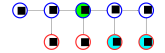
\includegraphics{figures/beta_example.pdf}
\caption[Beta]{The illustration of $\beta(x_2)=p(y_3,y_4|x_2)$}
\label{beta}
\end{figure}

\begin{figure}[b]
\includegraphics{figures/graphical_example.pdf}
\caption[Graphical Model]{The example of forward-backward}
\label{domaindecomp}
\end{figure}

\subsection{Likelihood function}
The sum of $p(x_t|\textbf{y})$ over the possible values of $x_t$ must equal one.
\begin{equation}
1 = \sum_{x_t} p(x_t|\textbf{y}) = \frac{\sum_{x_t} \alpha(x_t)\beta(x_t)}{p(\textbf{y})}
\end{equation}
So, the likelihood function $p(\textbf{y})$ can be written as
\begin{equation}
p(\textbf{y})=\sum_{x_t} \alpha(x_t)\beta(x_t)
\end{equation}

\subsection{Posterior probability $p(x_t | \textbf{y})$}
We denote the posterior probablity $p(x_t | \textbf{y})$ as $\gamma(x_t)$
\begin{equation}
\gamma(x_t) \triangleq \frac{\alpha(x_t)\beta(x_t)}{p(\textbf{y})}
\end{equation}

\subsection{Forward algorithm}
\begin{equation}
\alpha(x_{t+1}) = \sum_{x_t} \alpha(x_t) a_{x_t,x_{t+1}} p(y_{t+1}|x_{t+1})
\end{equation}
where $a_{x_t,x_{t+1}}$ is the transition probability from $x_t$ to $x_{t+1}$. The definition of alpha at the first time step yields:
\begin{equation}
\alpha(x_0) = p(y_0, x_0) = p(y_0|x_0)p(x_0) = p(y_0|x_0) \pi_{x_0} 
\end{equation}
and these values are used to initialize the recursion.

\subsection{Backward algorithm}
\begin{equation}
\beta(x_t) = \sum_{x_{t+1}} \beta(x_{t+1}) a_{x_t,x_{t+1}} p(y_{t+1}|x_{t+1})
\end{equation}
The beta recursion is a backwards recursion; that is, we start at the final time step $T$ and proceed backwards to the initial time step.

Some remarks:
\begin{enumerate}
\item $\beta(x_T)$ is unhelpful because it makes reference to a non-existent $y_{T+1}$
\item If we assign $\beta(x_T)$ to be a vector of ones, i.e., $\beta(x_T)=\textbf{1}$, we can compute $\beta(x_{T-1})$ correctly
\begin{equation}
\begin{split}
\beta(x_{T-1}) &= p(y_T|x_{T-1}) \\
&= \sum_{x_T} \beta(x_T) a_{x_{T-1}, x_T} p(y_T|x_T) \\
&= \sum_{x_T} a_{x_{T-1}, x_T} p(y_T|x_T) 
\end{split}
\end{equation}
\end{enumerate}

\subsection{Computing $p(\textbf{y})$ by a single forward pass for the alphas}
\begin{equation}
\begin{split}
p(\textbf{y}) &= \sum_{i} \alpha(x_T^i) \beta(x_T^i) \\
&= \sum_{i} \alpha(x_T^i) \\
&= \sum_{i} p(y_0,y_1,\cdots,y_T,x_T^i)
\end{split}
\end{equation}
\end{enumerate}


\section{Expectation maximization}
Preparing an initial potential mean force $V_0(x)$ and a diffusion coefficient $D_0$, and try to using the framework in the 2013 JPCB paper to learn $V(x)$ and $D$ back.

\section{Question}
\begin{enumerate}
\item If we ignore the information of photons, what is the observed data, $Y(t)$?
\item What is the likelihood functional?
\begin{equation}
\label{eq:PathP}
\begin{split}
\mathcal{P}(Y(t) ; F(x),D) &= \mathcal{P}(Y(t) ; \theta)= \mathcal{L}[\theta]\\
&=\langle \alpha_{t_0} |e^{-\bm{H}\Delta t_1}\bm{y}_1e^{-\bm{H}\Delta t_2}\bm{y}_2 \ldots e^{-\bm{H}\Delta t_{N_{\mathrm{P}}}}\bm{y}_{N_{\mathrm{P}}} | \beta_{t_{\mathrm{exp}}} \rangle
\end{split}
\end{equation}
\end{enumerate}

\section{Appendix A: Bayes' theorem}
\begin{equation}
p(A|B) = \frac{p(B|A)p(A)}{p(B)}
\end{equation}

\end{document}
